\chapter{Methodology}
\label{chapter:architecture}

\newenvironment{architecture}
{\quote\itshape}
{\endquote}

\begin{architecture}
\end{architecture}

\section{High Level Architecture}
\begin{figure}[h]
    \centering 
    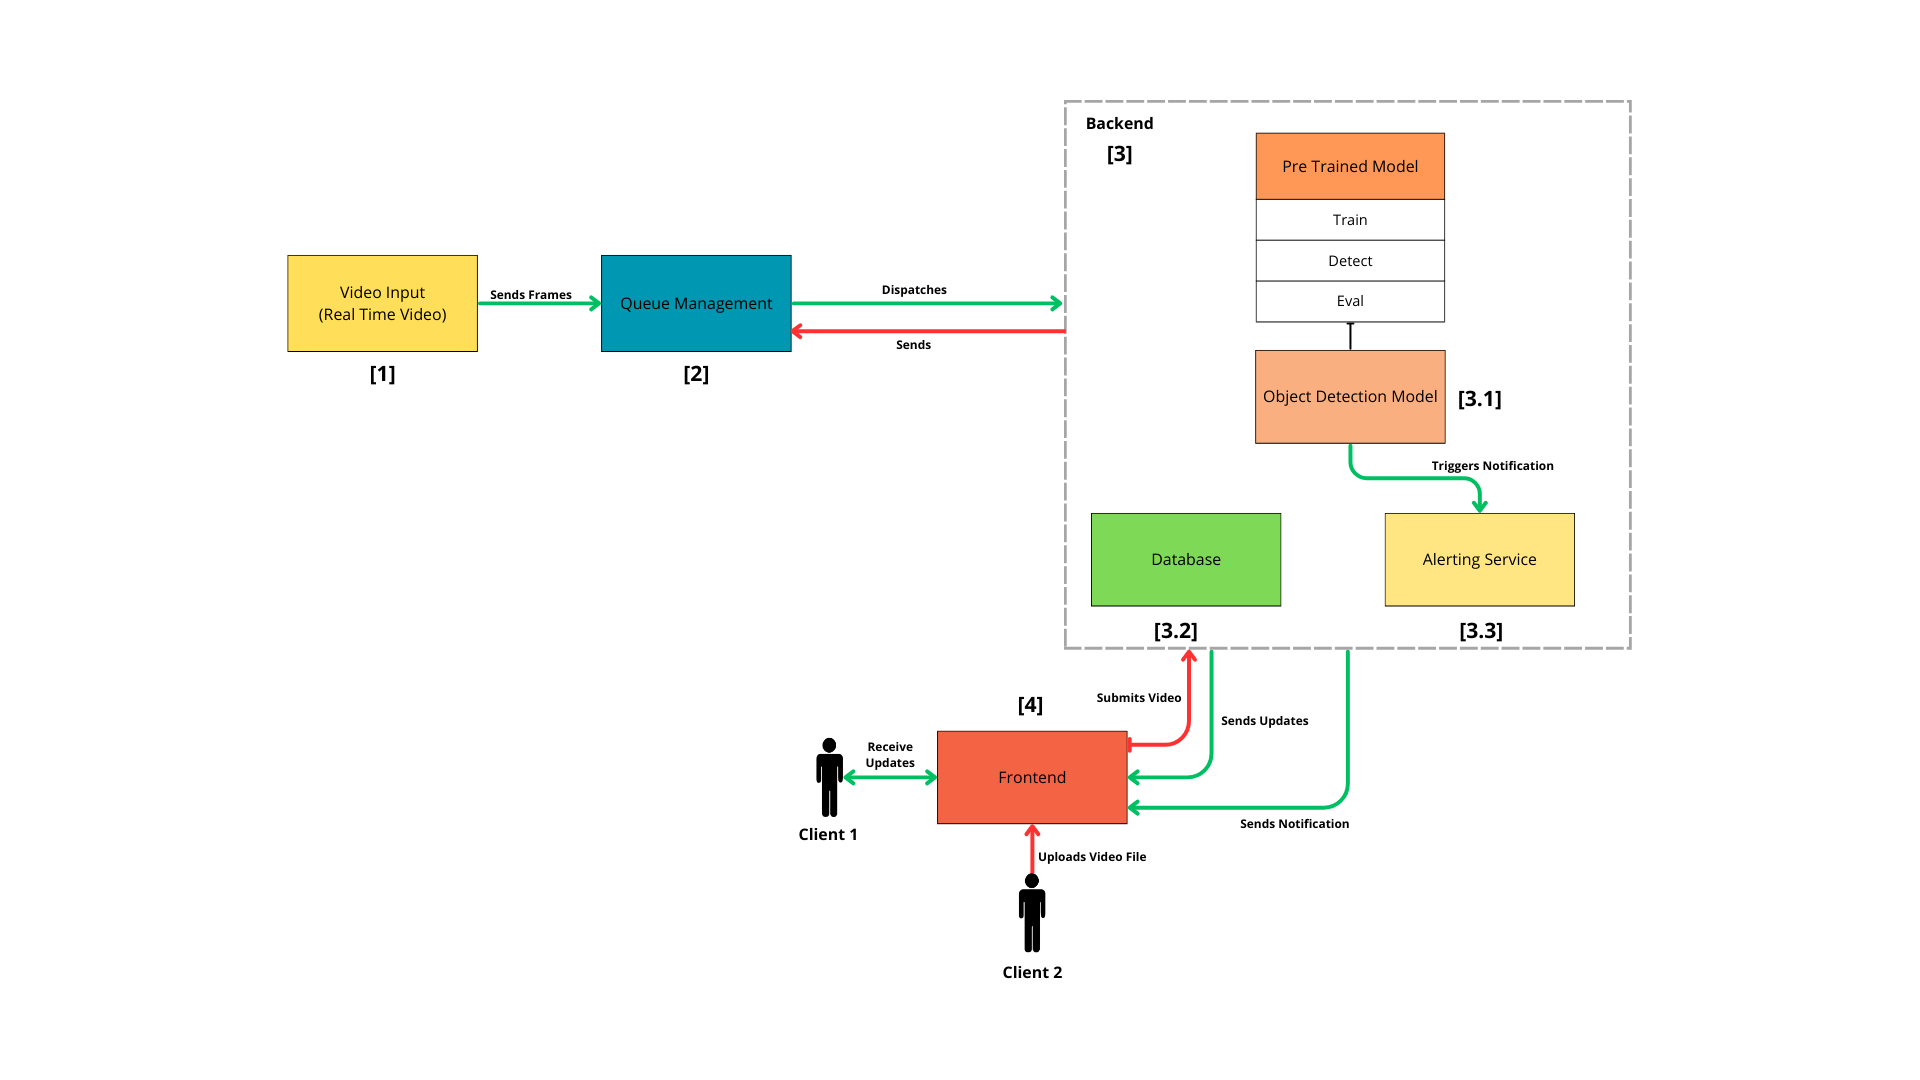
\includegraphics[width=\textwidth]{figs/architecture.png} 
    \caption{High Level Architecture Proposal}
    \label{fig:architecture-proposal}
\end{figure}

Figure \ref{fig:architecture-proposal} illustrates the proposed architecture for the system designed to automatically detect weapons. This system not only identifies weapons but also notifies relevant authorities upon detection. 

The Video Input (Real-Time Video) [1] consisting of CCTV cameras strategically installed across various locations, serves as the primary source of video data. These cameras are engineered to capture and transmit real-time video footage, which is then relayed frame by frame to the system for subsequent processing.

The Queue Management component [2] plays a key role in regulating the incoming data flow. It is specifically tasked with receiving video frames from the CCTV cameras and systematically queuing them for processing. This component is crucial for several reasons:
\begin{itemize}
    \item Load Balancing: effectively manages the influx of video frames, particularly crucial during periods of high input. Without this system, the backend could become overwhelmed, potentially leading to delays or processing failures.
    \item Prioritization: allows for the prioritization of certain video frames or streams, especially those from high-risk areas, ensuring they are processed earlier.
    \item Scalability: as the system expands to accommodate more video sources, Queue Management enables efficient scaling without necessitating significant modifications to the backend processing infrastructure.
\end{itemize}

The backend [3] serves as the system's central processing unit, encompassing a variety of integral modules:
\begin{itemize}
    \item Object Detection Model [3.1]: designed to identify objects of interest, primarily focusing on potentially dangerous items like firearms and knives. It operates with a pre-trained model, which has been finely tuned to pinpoint threats with precision.
    \item Database [3.2]: central to the system's functionality, the database is utilized for storing a wide range of critical data. This includes video metadata, logs of detected objects, model-related data, and other pertinent information that supports the system's operational integrity.
    \item Alerting Service [3.3]: key component of the system, playing a crucial role in ensuring safety. Upon detection of a hazardous object, it promptly generates notifications/alerts. These alerts are then swiftly relayed to the frontend, thereby enabling law enforcement officials to receive real-time updates and respond accordingly.
\end{itemize}

The frontend [4] constitutes a web interface, acting as the primary point of interaction for users, specifically law enforcement officers. They can upload video files directly through the frontend for subsequent analysis. Moreover, it serves as a dynamic platform for receiving timely updates and alerts regarding any detected objects, thereby streamlining the communication process and enhancing the efficiency of law enforcement responses.

\section{Work Plan and Milestones}